\documentclass[12pt]{beamer}

    \usepackage[utf8]{inputenc}
    \usepackage{graphics}
    \usepackage{listings}
    
    \usepackage{array,booktabs}
    
    \usetheme{Madrid}
    \usecolortheme{beaver}
    
    % custom commands
    \newcommand{\nologo}{\setbeamertemplate{logo}{}} % set logo to empty
    
    \title{Istio}
    \author{Arun}
    \date{\today}
    
    \begin{document}
        \begin{frame}
            \begin{center}
                \frametitle{What is Istio}
                \begin{itemize}
                    \pause
                    \item Service Mesh, Why do we need a Service Mesh?
                    \pause
                    \item Let's take an example
                \end{itemize}
            \end{center}
        \end{frame}

        \begin{frame}
            \begin{columns}
                \column{0.4\textwidth}
                    \begin{center}
                        \frametitle{bookinfo}
                        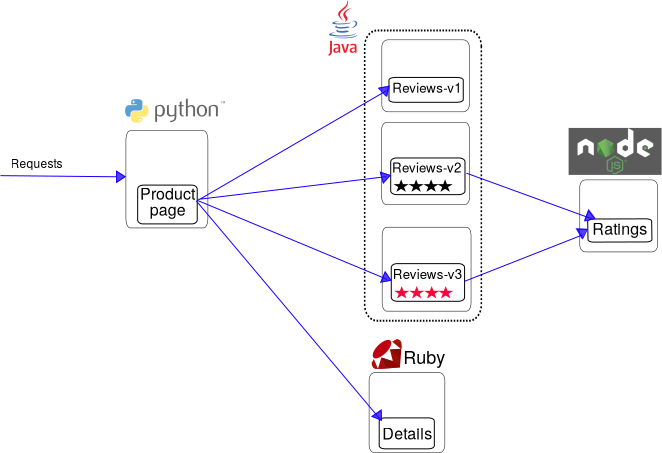
\includegraphics[width=1\textwidth]{images/bookinfo.png}
                    \end{center}

                \column{0.6\textwidth}
                    \begin{itemize}
                        \pause
                        \item Secure with mTLS
                        \pause
                        \item Connect
                        \pause
                        \item Service discovery, traffic management, test/canary versioning, incremental rollouts 
                        \pause
                        \item Retry policies, Circuit breaker
                        \pause
                        \item Observe
                        \pause
                        \item See where the bottlenecks are, how traffic flows
                        \pause
                        \item Control
                        \pause
                        \item Like who's allowed to talk to who, Rouge containers cannot talk to a service
                    \end{itemize}
            \end{columns}
        \end{frame}

        \begin{frame}
            \begin{columns}
                \column{0.4\textwidth}
                    \begin{center}
                        \frametitle{proxies}
                        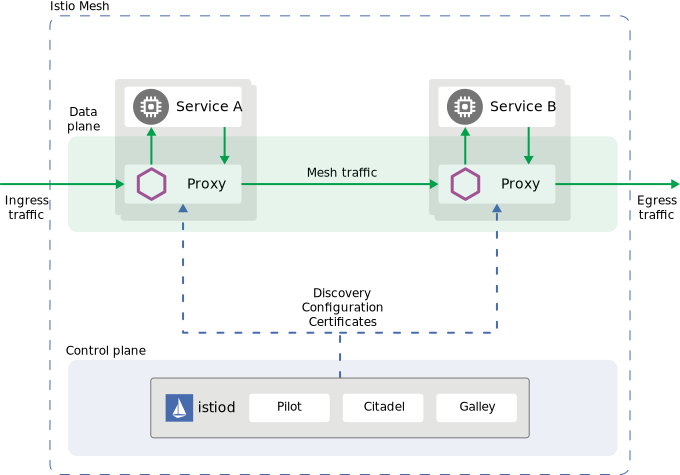
\includegraphics[width=1\textwidth]{images/proxies.png}
                    \end{center}

                    \column{0.6\textwidth}
                    \begin{itemize}
                        \pause
                        \item Injected envoy proxies to each containers in the system
                        \pause
                        \item It runs next to your containers in the same kuberneted pod
                        \pause
                        \item Intercepts all requests and responses, apply any policies defined
                    \end{itemize}
                \end{columns}
            \end{frame}

            \begin{frame}
                \begin{columns}
                    \column{0.4\textwidth}
                        \begin{center}
                            \frametitle{Istio tools}
                            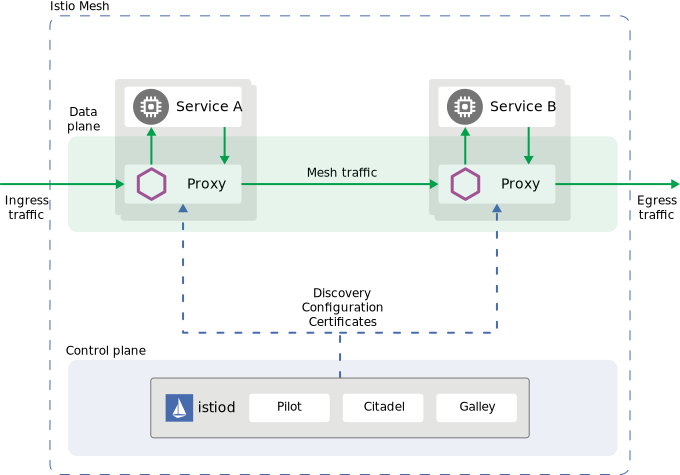
\includegraphics[width=1\textwidth]{images/proxies.png}
                        \end{center}
    
                        \column{0.6\textwidth}
                        \begin{itemize}
                            \pause
                            \item Galley
                            \pause
                            \item Pilot
                            \pause
                            \item Policy
                            \pause
                            \item Telemetry
                            \pause
                            \item Citadel
                        \end{itemize}
                    \end{columns}
                \end{frame}

                \begin{frame}
                    \begin{columns}
                        \column{0.4\textwidth}
                            \begin{center}
                                \frametitle{Istio Components}
                                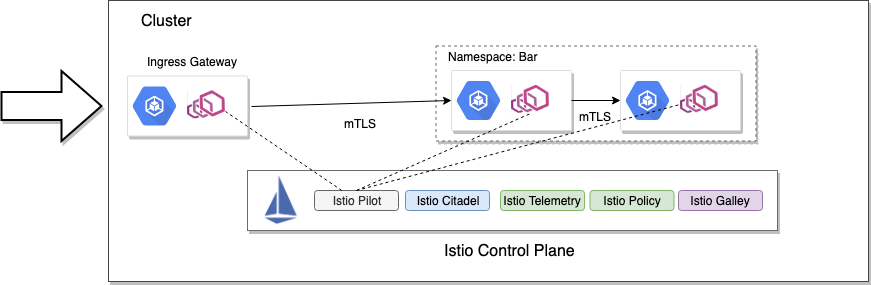
\includegraphics[width=1\textwidth]{images/components.png}
                            \end{center}
        
                            \column{0.6\textwidth}
                            \begin{itemize}
                                \pause
                                \item Gateway
                                \pause
                                \item Virtual Service
                                \pause
                                \item VS can be from Gateway to a service
                                \item VS can be from service to another service
                                \pause
                                \item VS is where u define the percentile trafic split for different versions
                                \pause
                                \item DestinationRules
                                \item For applying rules like Circuit breaker/retry/etc
                            \end{itemize}
                        \end{columns}
                    \end{frame}

                    \begin{frame}
                        \begin{itemize}
                            \item Let's do a demo
                        \end{itemize}        
                    \end{frame}
    
    \end{document}
